% Sección obligatoria 5: Implementación
% Fuentes: docs/pines.md, comun/*.h, nodo/src/main.cpp, gateway/src/main.cpp, bitacora_web.md.
\section{Implementación}
\label{sec:implementacion}

\subsection{Hardware e interconexiones}
\label{sec:interconexiones}

La Fig.~\ref{fig:interconexiones} muestra cómo se conectan los módulos al ESP32 del nodo. Los tres sensores analógicos usan canales del ADC1, que el ESP32 puede leer mientras el Wi-Fi está activo~\cite{esp32}. Las salidas del pH y de la turbidez se alimentan con 5~V y pueden superar los 3.3~V que admite un pin del ESP32. Por eso pasan por un divisor de 10~k$\Omega$ (arriba) y 20~k$\Omega$ (abajo), que entrega dos tercios de la tensión. El TDS se alimenta con 3.3~V y su salida, de 0 a 2.3~V, se conecta directamente. El DS18B20 comparte un bus 1-Wire con una resistencia de 4.7~k$\Omega$ a 3.3~V. El RAK3272S se alimenta del pin de 3.3~V del ESP32 y se comunica por el segundo puerto serie, con las líneas TX y RX cruzadas (\texttt{docs/pines.md}).

En el lado de potencia hay dos dominios. El nodo se alimenta por USB desde el computador, que también recibe la salida serie usada como evidencia. El segundo dominio es un módulo HW-131 conectado a una fuente de 8~V y 2~A. De sus rieles de 5~V y 3.3~V se alimentan los sensores y la bobina del relé, y a través del contacto normalmente abierto del relé, la bomba. El ESP32 y el HW-131 comparten tierra, porque el ESP32 lee señales de sensores alimentados desde el HW-131. El relé conmuta con nivel bajo en GPIO23. Por eso el firmware fija ese pin en alto antes y después de configurarlo como salida, para que la bomba no arranque durante el encendido. Se usa uno de los dos canales de un módulo de relé.

En las primeras pruebas, el ESP32 se desconectaba del puerto USB del computador cada vez que el relé conmutaba la bomba. Primero se probó un diodo 1N4007 en paralelo con el motor (7 de noviembre). En el montaje final ese diodo ya no está: el problema se resolvió separando la alimentación de la bobina del relé. Para eso se retiró el puente \texttt{JD-VCC}/\texttt{VCC} del módulo, de modo que la bobina se alimenta desde los 5~V del HW-131 y el ESP32 solo aporta \texttt{VCC} y la señal \texttt{IN2}. Además, se colocó un capacitor electrolítico de 220~$\mu$F entre \texttt{JD-VCC} y \texttt{GND}, junto al módulo, para absorber el pico de corriente al energizar la bobina. El módulo trae su propio diodo en paralelo con la bobina, que protege al transistor que la maneja, pero no hay diodo en paralelo con el motor de la bomba. Estas observaciones son del equipo y no tienen un log asociado (Sección~\ref{sec:resultados}).

\begin{figure}[htbp]
\centering
\resizebox{\textwidth}{!}{%
\begin{tikzpicture}[
    mod/.style={box, text width=34mm, minimum height=11mm},
    pwr/.style={box, text width=34mm, minimum height=11mm, fill=white, draw=power},
    div/.style={rectangle, draw=navy, fill=white, font=\scriptsize, align=center, inner sep=1.5pt, minimum height=7mm},
    pin/.style={font=\scriptsize\ttfamily, inner sep=1pt, fill=white},
    lab/.style={font=\scriptsize, inner sep=1pt, fill=white}
]
% ESP32 central
\node[box, fill=navy, text=white, text width=36mm, minimum height=78mm, font=\small] (esp) at (0,0) {ESP32 DevKit V1\\(nodo QM01)};

% Sensores (izquierda)
\node[mod] (ph)   at (-7.6, 3.0)  {pH DFRobot SEN0169\\(5 V del HW-131)};
\node[mod] (turb) at (-7.6, 1.0)  {Turbidez TS-300B\\(5 V del HW-131)};
\node[mod] (tds)  at (-7.6,-1.0)  {TDS KS0429 (3.3 V, HW-131)\\salida 0--2.3 V directa};
\node[mod] (temp) at (-7.6,-3.0)  {DS18B20\\(3.3 V, HW-131; 1-Wire)};
\node[div] (dph)  at (-3.7, 3.0)  {divisor\\10k/20k};
\node[div] (dtu)  at (-3.7, 1.0)  {divisor\\10k/20k};
\node[div] (pu)   at (-3.7,-3.0)  {pull-up\\4.7k a 3V3};

\draw[arr] (ph) -- (dph);   \draw[arr] (dph) -- node[pin, above]{GPIO33} (esp.west |- dph);
\draw[arr] (turb) -- (dtu); \draw[arr] (dtu) -- node[pin, above]{GPIO34} (esp.west |- dtu);
\draw[arr] (tds) -- node[pin, pos=0.8, above]{GPIO35} (esp.west |- tds);
\draw[arr, <->] (temp) -- (pu); \draw[arr, <->] (pu) -- node[pin, above]{GPIO32} (esp.west |- pu);

% Radio, relé y E/S (derecha)
\node[mod] (rak)  at (6.9, 3.0)  {RAK3272S\\(3.3 V desde el ESP32)};
\node[mod] (rele) at (6.9, 0.6)  {Relé, canal 2 de 2\\(bobina a 5 V del HW-131, 220 $\mu$F)};
\node[mod] (led)  at (6.9,-3.4)  {LED testigo};

\draw[arr] ($(esp.east |- rak)+(0,0.25)$) -- node[pin, above]{GPIO17 (TX2) $\to$ RX} ($(rak.west)+(0,0.25)$);
\draw[arr] ($(rak.west)+(0,-0.25)$) -- node[pin, below]{GPIO16 (RX2) $\gets$ TX} ($(esp.east |- rak)+(0,-0.25)$);
\draw[arr] (esp.east |- rele) -- node[pin, above]{GPIO23} (rele);
\draw[arr] (esp.east |- led) -- node[pin, above]{GPIO2} (led);

% Potencia
\node[pwr] (usb)  at (0,-5.6)   {USB del computador\\(alimentación y registro)};
\node[pwr] (hw)   at (6.9, 6.0) {Fuente 8 V 2 A\\+ módulo HW-131};
\node[box, text width=24mm, minimum height=11mm] (bomba) at (11.0, 0.6) {Minibomba\\sumergible};
\draw[energy] (usb) -- (esp.south);
\draw[energy] (hw.east) -| node[lab, pos=0.75, right]{vía contacto NO} (bomba.north);
\draw[energy] (rele) -- (bomba);
\draw[energy] (hw.west) -| node[lab, pos=0.2, above]{rieles 5 V y 3.3 V a sensores y bobina} (ph.north);
\draw[arr, <->] (rak.north) -- ++(0,0.5) node[lab, above]{antena 923.5 MHz};
\end{tikzpicture}%
}
\caption{Interconexiones del nodo QM01 con los pines del firmware final (\texttt{nodo/src/main.cpp}, \texttt{comun/hardware.h}). Azul: señales; naranja discontinuo: alimentación. El gateway GW01 usa la misma conexión ESP32--RAK3272S (GPIO16/17). Elaboración propia.}
\label{fig:interconexiones}
\end{figure}

\subsection{Firmware del nodo QM01}
\label{sec:fw_nodo}

El firmware del nodo es un solo lazo que nunca se bloquea (Fig.~\ref{fig:flujo_nodo}). En cada vuelta alimenta al \textit{watchdog}, atiende los comandos del puerto serie, supervisa el tiempo de la bomba y evalúa la solicitud de rearme. Cada 5~s, medidos sin deriva acumulada, ejecuta un ciclo de adquisición. Mientras la bomba funciona no se leen sensores ni se usa el radio: el lazo solo vigila el corte de la bomba.

\begin{figure}[htbp]
\centering
\resizebox{!}{0.80\textheight}{%
\begin{tikzpicture}[
    node distance=6mm,
    pb/.style={box, text width=44mm, minimum height=9mm},
    dc/.style={decision, text width=30mm, aspect=2.4},
    lab/.style={font=\scriptsize, inner sep=1pt, fill=white}
]
\node[term] (ini) {Encendido};
\node[pb, below=of ini] (setup) {Relé OFF; abrir NVS; recuperar estado (Fig.~\ref{fig:fsm}); configurar RAK; armar TWDT 5000 ms};
\node[pb, below=of setup] (base) {Alimentar \textit{watchdog}; leer comandos serie; supervisar bomba; atender rearme};
\node[dc, below=of base] (ta) {¿Pasaron 5 s?};
\node[dc, below=9mm of ta] (mue) {¿Estado = MUESTREANDO?};
\node[pb, below=9mm of mue] (leer) {Leer sensores: mediana de 31 muestras; DS18B20 asíncrono; validez por canal};
\node[pb, below=of leer] (det) {Detector: umbrales, contadores de persistencia, TDS$_0$ automático};
\node[dc, below=of det] (sol) {¿Solicitud de captura y ARMADO?};
\node[pb, right=18mm of sol] (cap) {Guardar \texttt{bloqueado}, \texttt{bombeando} en NVS $\to$ trama MUESTREANDO $\to$ relé ON};
\node[pb, below=9mm of sol] (tx) {Armar trama de 27 bytes con CRC-16 y enviar con \texttt{AT+PSEND}};
\node[dc, below=of tx] (ce) {¿Estado = CAPTURA\_ ESTIMADA?};
\node[pb, right=18mm of ce] (blo) {Pasar a BLOQUEADO};

\coordinate (ret) at ($(base.west)+(-14mm,0)$);
\draw[arr] (ini) -- (setup);
\draw[arr] (setup) -- (base);
\draw[arr] (base) -- (ta);
\draw[arr] (ta) -- node[lab, right]{sí} (mue);
\draw[arr] (mue) -- node[lab, right]{no} (leer);
\draw[arr] (leer) -- (det);
\draw[arr] (det) -- (sol);
\draw[arr] (sol) -- node[lab, above]{sí} (cap);
\draw[arr] (sol) -- node[lab, right]{no} (tx);
\draw[arr] (tx) -- (ce);
\draw[arr] (ce) -- node[lab, above]{sí} (blo);
\draw[arr] (ta.west) -- node[lab, above]{no} (ta.west -| ret) -- (ret) -- (base.west);
\draw[arr] (mue.west) -- node[lab, above]{sí} (mue.west -| ret);
\draw[arr] (ce.west) -- node[lab, above]{no} (ce.west -| ret) -- (ret);
\draw[arr] (cap.north) |- ($(base.east)+(0,0)$);
\draw[arr] (blo.east) -- ++(6mm,0) |- (cap.north |- base.east);
\end{tikzpicture}%
}
\caption{Diagrama de flujo del lazo principal del nodo QM01, según \texttt{nodo/src/main.cpp}. Elaboración propia.}
\label{fig:flujo_nodo}
\end{figure}

\textbf{Trama.} Cada ciclo produce una trama binaria de 27 bytes definida en \texttt{comun/trama.h}, archivo que comparten el nodo y el gateway (Tabla~\ref{tab:trama}). El valor de cada canal se transmite como entero escalado. Si el bit de validez del canal es 0, se envía el centinela $-32768$. Al final se agrega un CRC-16/CCITT-FALSE (polinomio \texttt{0x1021}, valor inicial \texttt{0xFFFF}). El número de secuencia permite detectar pérdidas y duplicados, y el contador de reinicios (\texttt{boot\_id}) distingue una secuencia nueva de una repetida.

\begin{table}[htbp]
\centering
\small
\caption{Campos de la trama LoRa de 27 bytes (\texttt{comun/trama.h})}
\label{tab:trama}
\begin{tabularx}{\textwidth}{l c Y}
\toprule
Campo & Bytes & Contenido \\
\midrule
\texttt{version}, \texttt{nodo\_id} & 1 + 1 & Versión del formato (1) e identificador del nodo (1 = QM01) \\
\texttt{boot\_id} & 2 & Contador de reinicios guardado en NVS \\
\texttt{seq}, \texttt{t\_ms} & 4 + 4 & Número de secuencia y milisegundos desde el encendido \\
\texttt{ph\_x100}, \texttt{tds\_ppm}, \texttt{it\_x1000}, \texttt{temp\_x100} & 2 + 2 + 2 + 2 & Mediciones escaladas a enteros \\
\texttt{validez}, \texttt{anomalias}, \texttt{estado} & 1 + 1 + 1 & Bits por canal (pH 0x01, TDS 0x02, turbidez 0x04, temperatura 0x08) y estado de la FSM \\
\texttt{evento\_id} & 2 & Identificador de la última captura \\
\texttt{crc} & 2 & CRC-16/CCITT-FALSE de los 25 bytes anteriores \\
\bottomrule
\end{tabularx}
\end{table}

\textbf{Radio.} El módulo RAK3272S se configura con \texttt{AT+NWM=0} (modo punto a punto) y \texttt{AT+P2P} (parámetros de la Sección~\ref{sec:cambios}). La trama se envía en hexadecimal con \texttt{AT+PSEND}, y el envío se da por terminado cuando el módulo responde \texttt{+EVT:TXP2P DONE} (\texttt{comun/rak\_at.h}). Si el radio falla, el nodo marca la trama como no enviada y sigue funcionando. La captura de la muestra no depende del radio.

\textbf{\textit{Watchdog}.} El nodo usa el \textit{watchdog} de tareas del ESP32 (TWDT) con un plazo de 5000~ms y reinicio automático. Se arma después de configurar el RAK, cuyos comandos AT pueden tardar, y se alimenta una vez por vuelta del lazo. Al arrancar, el nodo imprime el motivo del reinicio. En la prueba de control sin fallas forzadas, la vuelta más larga del lazo (\texttt{loop\_max\_ms}) estuvo entre 169 y 180~ms, cerca del 3.6~\% del plazo (\texttt{nodo\_20261112\_150625\_wdt\_control.log}). Si el reinicio ocurre a mitad de un bombeo, el nodo arranca en \texttt{FALLO} (Sección~\ref{sec:reglas}).

\subsection{Firmware del gateway GW01 y supervisión por MQTT}
\label{sec:fw_gateway}

El gateway deja su RAK3272S en recepción continua (\texttt{AT+PRECV=65534}) y procesa cada evento \texttt{+EVT:RXP2P} que trae el RSSI, la SNR y la trama (\texttt{gateway/src/main.cpp}). Para cada trama recibida el gateway hace lo siguiente:
\begin{enumerate}
    \item Convierte la trama de hexadecimal a binario y descarta las que tienen una versión desconocida o un CRC incorrecto.
    \item Identifica el nodo por su \texttt{nodo\_id} y descarta los duplicados por número de secuencia. Si cambia el \texttt{boot\_id}, reinicia las estadísticas de ese nodo y calcula el PDR acumulado del arranque actual.
    \item Arma la telemetría en JSON con las mediciones, la validez, las anomalías, el estado, el evento, la secuencia, el RSSI, la SNR y el PDR. Omite las cuatro mediciones cuyo bit de validez es 0, para que el centinela no llegue al tablero como si fuera un dato.
    \item Si la hora ya se sincronizó por NTP, añade la marca de tiempo absoluta en milisegundos.
    \item Publica por MQTT en tópicos jerárquicos del tipo \ev{qawapmayu/v1/<zona>/<sitio>/<nodo>/<canal>}, con mensajes retenidos para que un cliente que se conecta reciba de inmediato el último valor. La telemetría pasa por una cola circular de 16 posiciones.
\end{enumerate}

Además de \texttt{telemetria}, cada nodo tiene canales de \texttt{estado} (se publica solo cuando cambia), \texttt{evento} (cada captura nueva), \texttt{enlace} (RSSI, SNR y PDR), \texttt{meta} (nombre y coordenadas) y \texttt{conexion}. El gateway se conecta al broker con un mensaje de última voluntad (LWT). Si el gateway se cae, el propio broker publica \texttt{fuera\_de\_linea} en su tópico de conexión. Si un nodo pasa 30~s sin enviar tramas, el gateway lo marca fuera de línea.

El gateway también cubre dos fallas. La primera es la caída de la red: el Wi-Fi intenta reconectarse cada 10~s y la cola conserva la telemetría mientras tanto. A razón de una trama cada 5~s, 16 posiciones cubren unos 80~s sin red; después se descarta el mensaje más antiguo. Los canales de estado, evento y enlace no se encolan: al reconectar se republica el último valor. La segunda falla es la ``sordera'' del RAK, cuando el módulo deja de entregar tramas sin causa conocida. Si pasan 60~s sin recibir una trama, el gateway vuelve a configurar el RAK en recepción. Tras tres intentos sin éxito, reinicia el ESP32. Cada paso de esta recuperación se publica en el tópico de diagnóstico del gateway. El gateway no tiene \textit{watchdog}.

\textbf{Broker y tablero.} Hasta el 12 de noviembre la telemetría se envió a ThingsBoard Cloud~\cite{thingsboard}, donde el dispositivo QM01 tenía tarjetas, gráficos, una tabla de historial y una alarma de anomalía persistente. El 13 de noviembre se reemplazó por una cadena propia, para no depender de la cuota de una plataforma externa y controlar por completo la presentación:
\begin{itemize}
    \item \textbf{Broker:} Mosquitto en la laptop, con MQTT en el puerto 1883 para el gateway y WebSockets en el 9001 para el navegador (\texttt{broker/}). Para una demostración por Internet puede usarse un broker público; en ese caso, cualquiera que conozca el tópico puede leer los datos.
    \item \textbf{Tablero:} página web estática (\texttt{tablero/}) que se suscribe al broker por WebSockets. Tiene cuatro vistas: Monitoreo (gráficos por estación y mapa de cobertura), Eventos (estado de conexión, enlace y sordera), un inspector de mensajes MQTT y la configuración de conexión. Las librerías van incluidas en el repositorio, así que funciona sin Internet dentro de la red local.
    \item \textbf{Herramientas:} un simulador de dos nodos adicionales permite probar el tablero con varias estaciones, y un registrador (\texttt{herramientas/registro\_mqtt.py}) guarda en CSV cada mensaje que pasa por el broker. Esos CSV son la evidencia de la Sección~\ref{sec:res_integral}.
\end{itemize}

\begin{figure}[htbp]
\centering
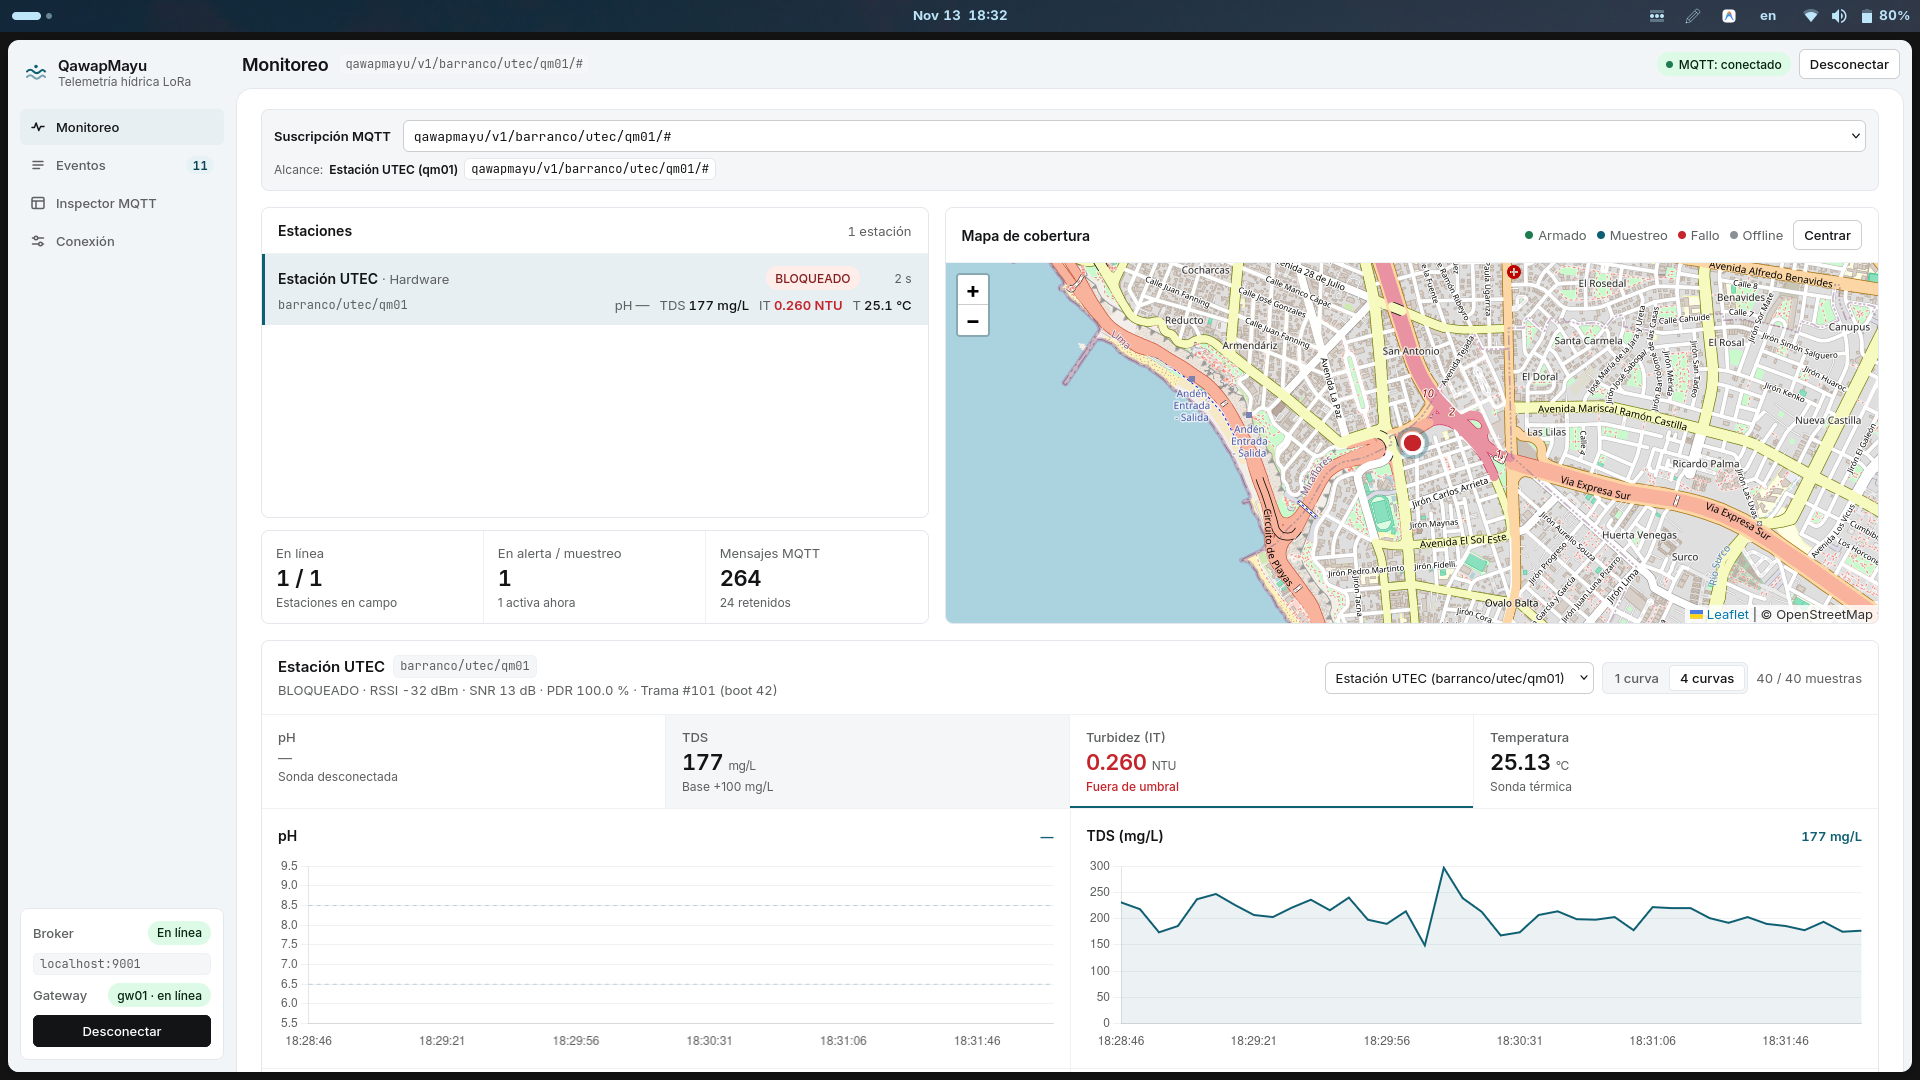
\includegraphics[width=\textwidth]{figuras/dashboard.png}
\caption{Tablero web propio, vista Monitoreo, el 13 de noviembre de 2026 a las 18:32, poco después de la cuarta captura del ensayo integral. Muestra el broker y el gateway en línea, la estación QM01 en BLOQUEADO con RSSI de $-32$~dBm y PDR del 100~\%, el mapa de cobertura y las series de pH (sonda desconectada) y TDS. La etiqueta ``NTU'' que el tablero muestra junto a la turbidez corresponde en realidad al índice adimensional $I_T$. El nombre ``Estación UTEC'' y su posición en el mapa son valores de ejemplo configurados en el gateway; el ensayo se hizo en un domicilio. Elaboración propia.}
\label{fig:dashboard}
\end{figure}

\subsection{Organización del software y trazabilidad de la evidencia}
\label{sec:software}

El software está en un repositorio Git y se compila con PlatformIO, con la plataforma fijada en \texttt{espressif32@8.0.0} (núcleo Arduino-ESP32 3.3.12) para que todas las compilaciones sean reproducibles. El código se organiza en cuatro partes:
\begin{itemize}
    \item \texttt{comun/}: cabeceras compartidas por todos los firmwares. Contiene el formato de la trama y el CRC (\texttt{trama.h}), el detector de anomalías y la validez (\texttt{anomalia.h}), el manejo del RAK por comandos AT (\texttt{rak\_at.h}), los pines (\texttt{hardware.h}) y la recta de pH (\texttt{calibracion.h}). Al compartirlas, el nodo y el gateway no pueden discrepar en el formato de la trama.
    \item \texttt{nodo/} y \texttt{gateway/}: los dos firmwares finales. Las credenciales de Wi-Fi y de ThingsBoard están en un archivo que Git ignora, así que no forman parte del repositorio.
    \item \texttt{herramientas/}: firmwares de banco usados para probar cada parte por separado: \texttt{sensores}, \texttt{bomba\_manual}, \texttt{fsm\_led}, \texttt{rele\_arranque} y \texttt{puente\_rak}.
    \item \texttt{herramientas/monitor/filter\_evidencia.py}: filtro del monitor serie que guarda cada prueba en \texttt{pruebas/} como \texttt{.log} o \texttt{.csv}, con fecha, hora y nombre de la prueba.
\end{itemize}
Cada cambio de código y cada lote de evidencia quedó en su propio commit, de modo que cada resultado de la Sección~\ref{sec:resultados} puede rastrearse hasta la versión del firmware que lo produjo.

\subsection{Armado del prototipo}
\label{sec:armado}

El nodo se montó en una caja plástica con perforaciones laterales para los cables de las sondas, el USB y la manguera (Fig.~\ref{fig:fotos_nodo}). Dentro de la caja, los módulos acondicionadores, el relé y el microcontrolador van fijos a la base, y las conexiones se reparten con una protoboard. La antena del RAK3272S queda fuera de la caja. El montaje hidráulico cambió a lo largo de las pruebas. En la serie de dosificación del 8 de noviembre la bomba estaba sumergida en la fuente (Fig.~\ref{fig:foto_g1}; geometría G1, Sección~\ref{sec:res_dosif}). Para el ensayo integral se sacó la bomba del agua (Fig.~\ref{fig:acople}). El recipiente de prueba tiene una salida en su pared, cerca del fondo, y un acople rápido lleva el agua por gravedad hasta la entrada de la bomba, que queda sobre la mesa. Así la bomba no comparte el recipiente con los sensores y se puede retirar sin vaciarlo. El agua sigue atravesando la bomba, de modo que la muestra no queda aislada de ella.

\begin{figure}[htbp]
\centering
\begin{minipage}[b]{0.40\textwidth}
\centering
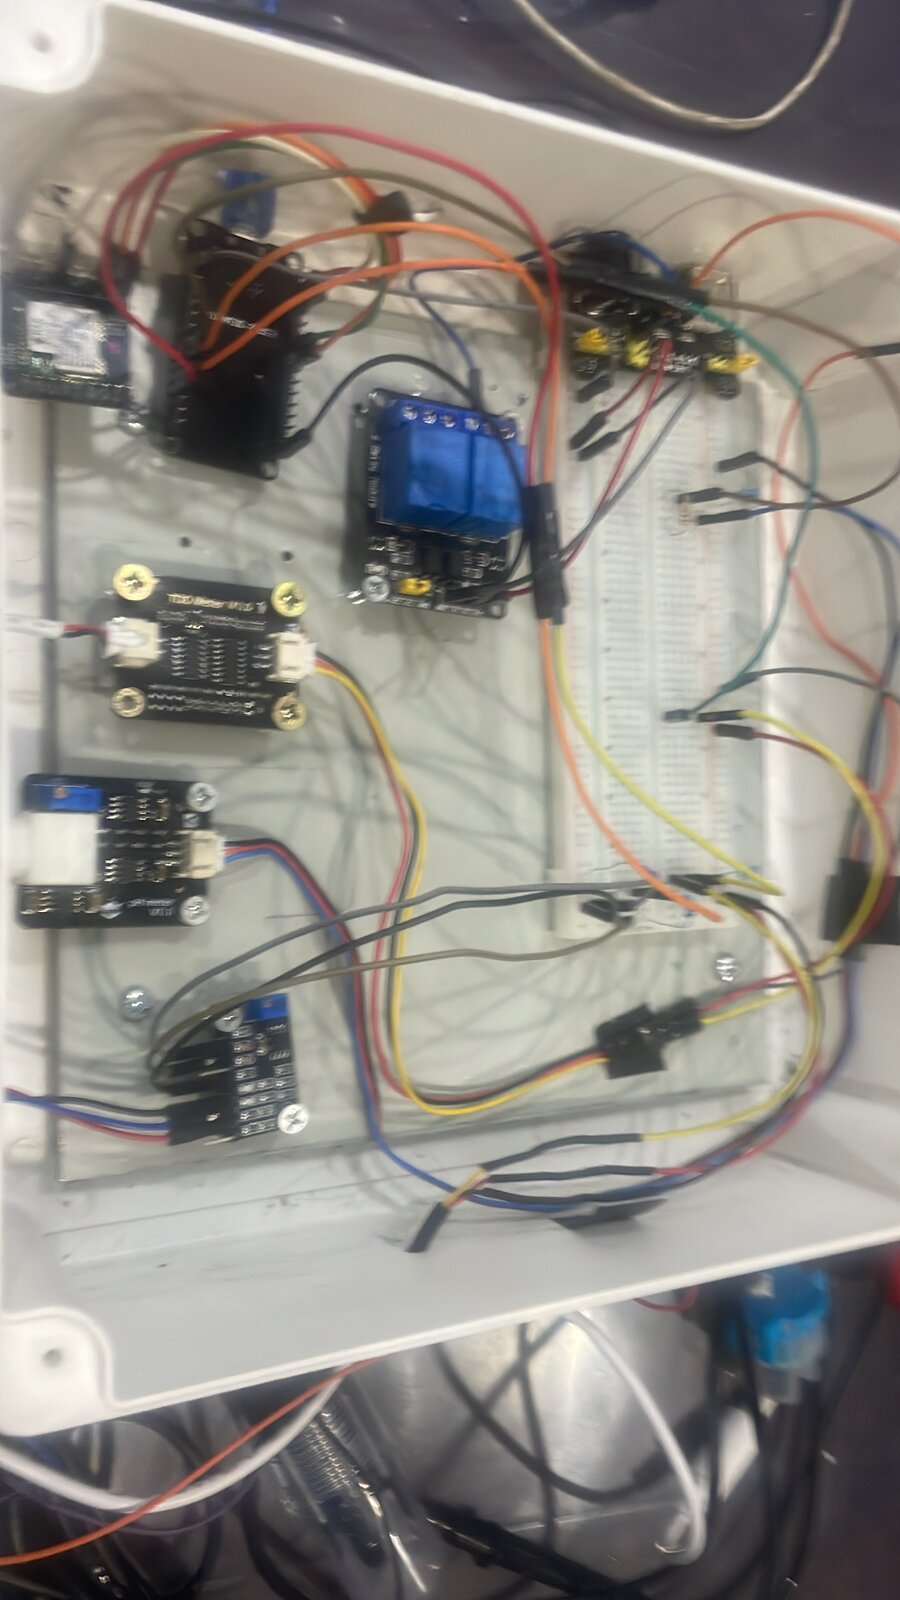
\includegraphics[width=\linewidth,height=8cm,keepaspectratio]{figuras/fotos/nodo_vista_superior.jpg}\\
\small (a) Vista superior del interior de la caja.
\end{minipage}\hfill
\begin{minipage}[b]{0.56\textwidth}
\centering
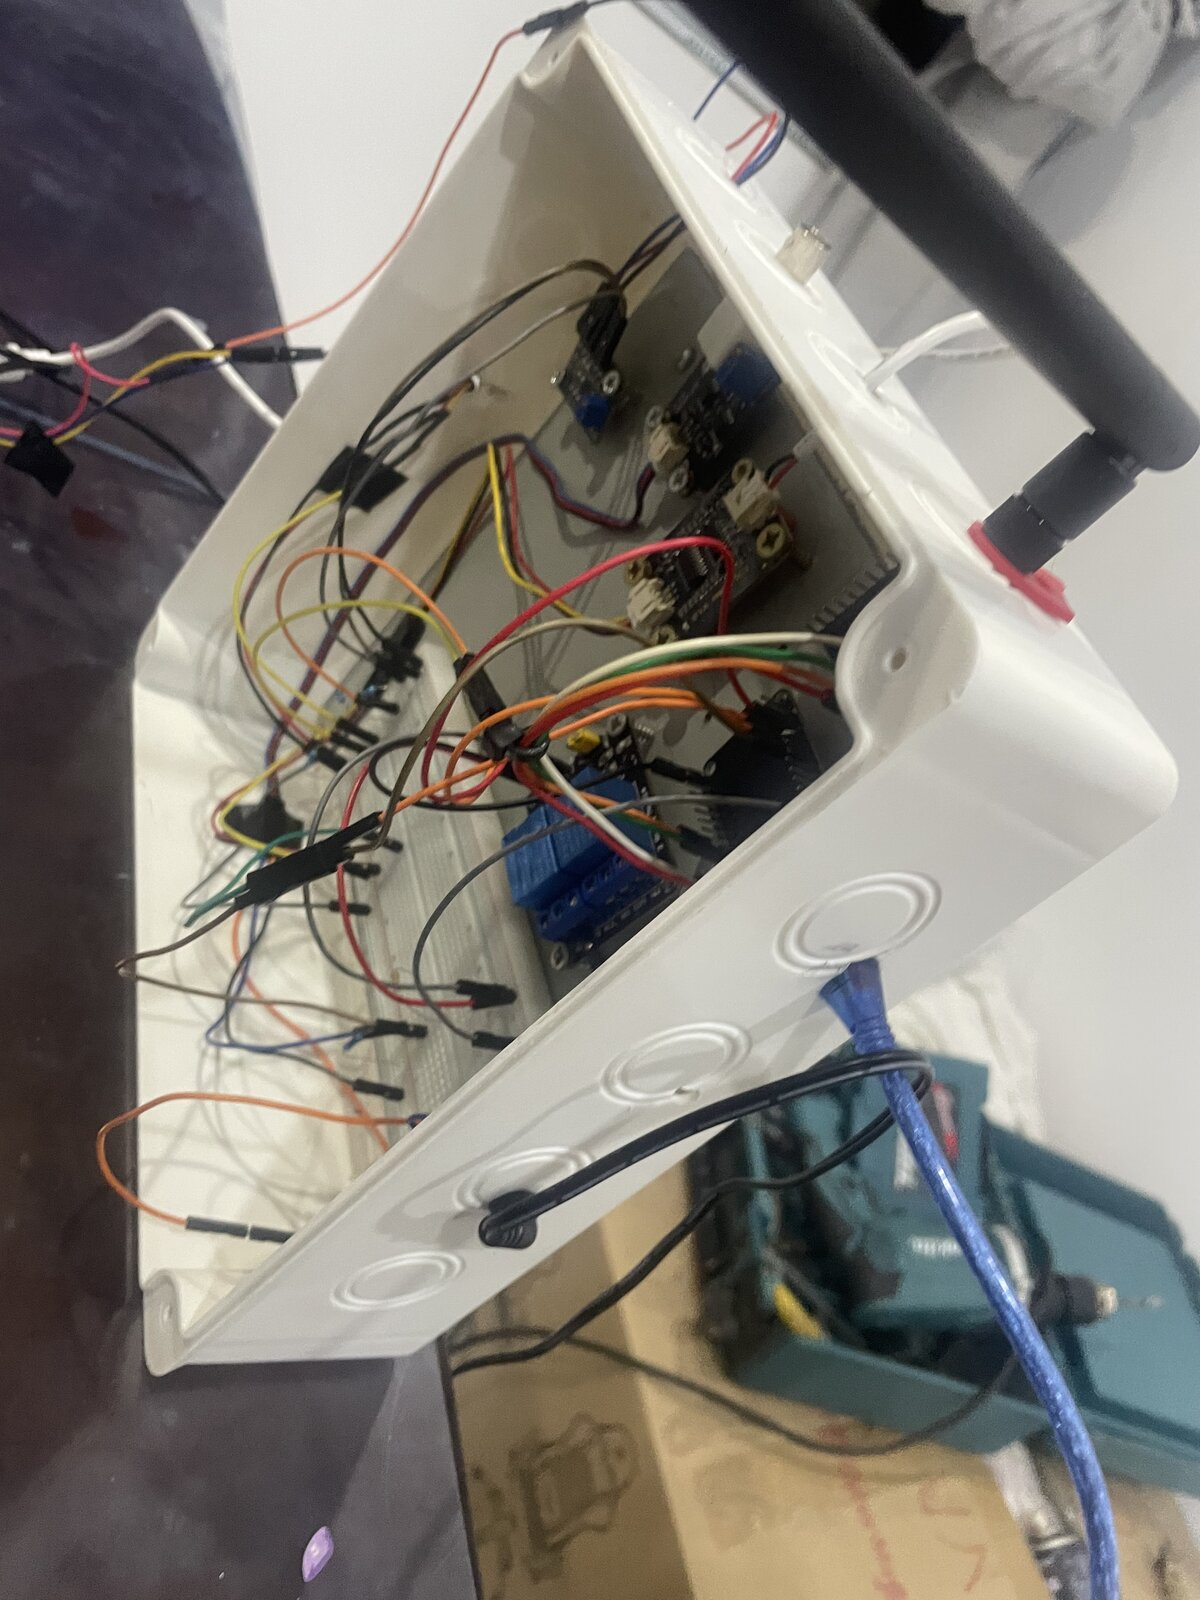
\includegraphics[width=\linewidth,height=8cm,keepaspectratio]{figuras/fotos/nodo_con_antena.jpg}\\
\small (b) Caja con la antena del RAK3272S y el cable USB.
\end{minipage}
\caption{Nodo QM01 armado (fotografías del 12 de noviembre de 2026). Elaboración propia.}
\label{fig:fotos_nodo}
\end{figure}

\begin{figure}[htbp]
\centering
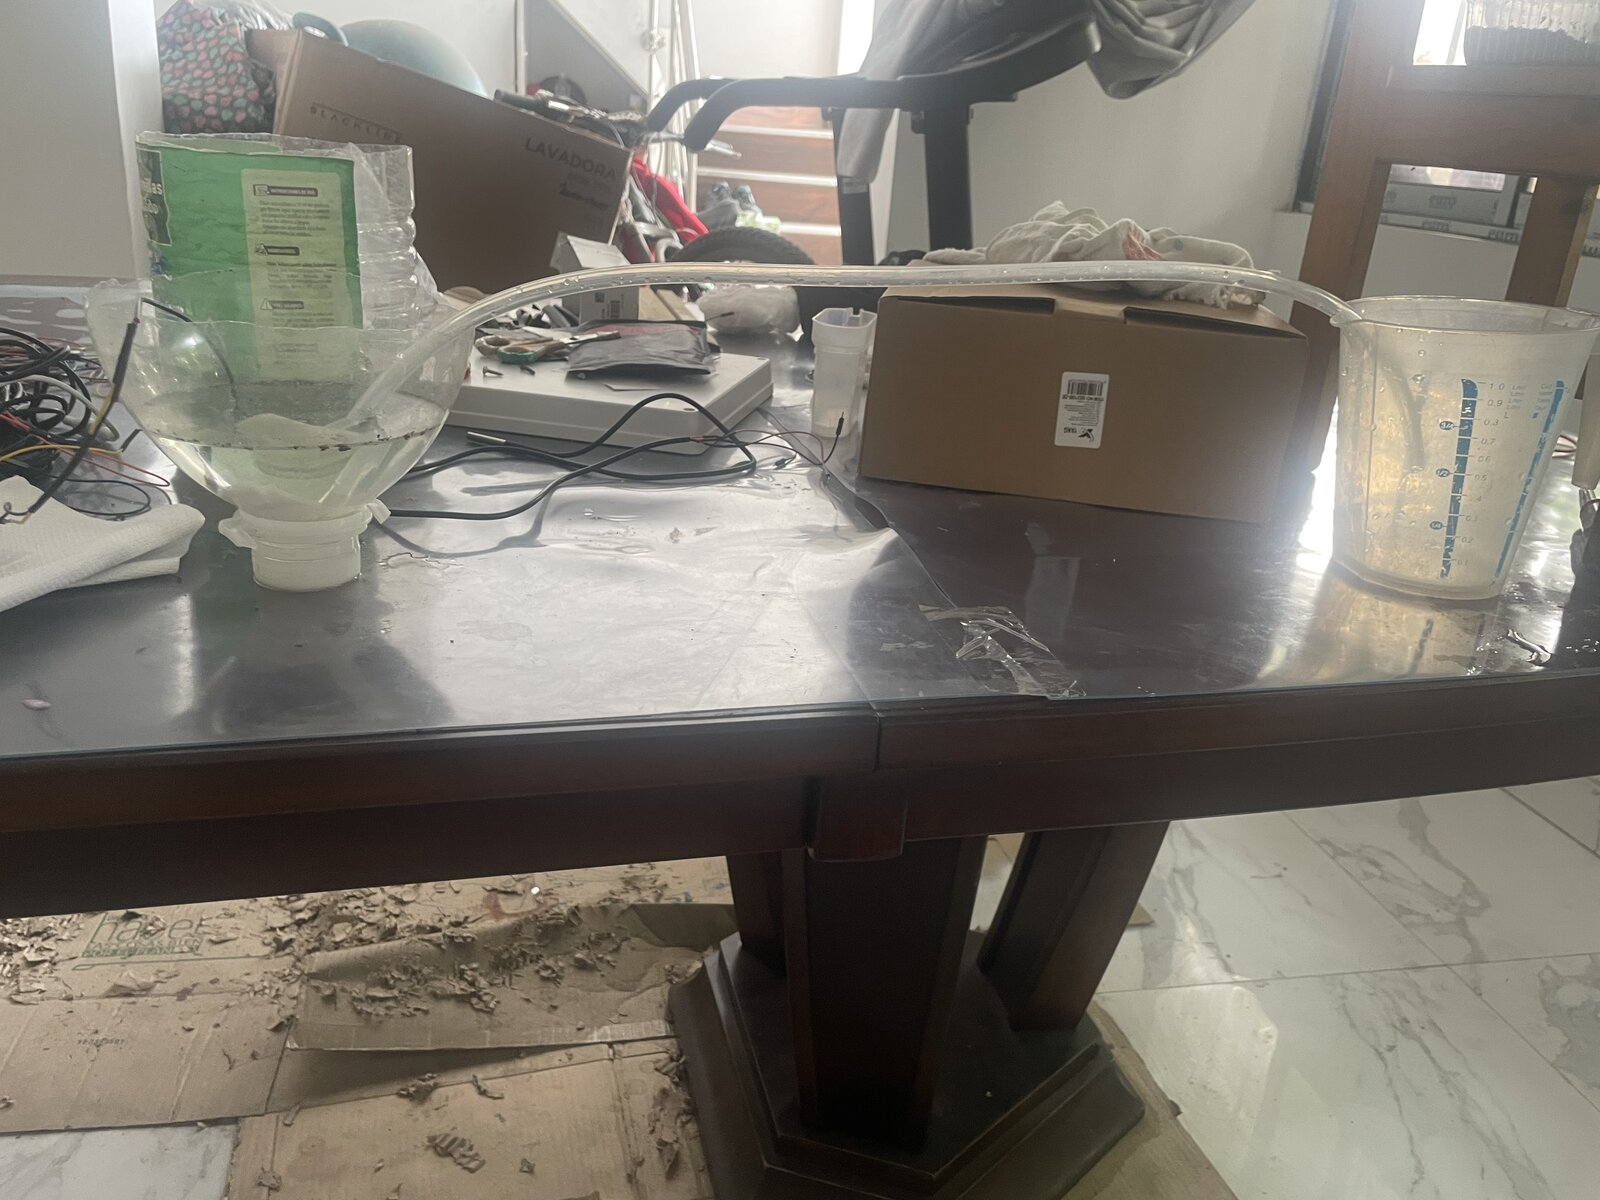
\includegraphics[width=0.75\textwidth]{figuras/fotos/dosificacion_G1.jpg}
\caption{Montaje de la serie de dosificación del 8 de noviembre de 2026: manguera de 70 cm con su tramo horizontal entre la fuente y el frasco graduado. Elaboración propia.}
\label{fig:foto_g1}
\end{figure}

\begin{figure}[htbp]
\centering
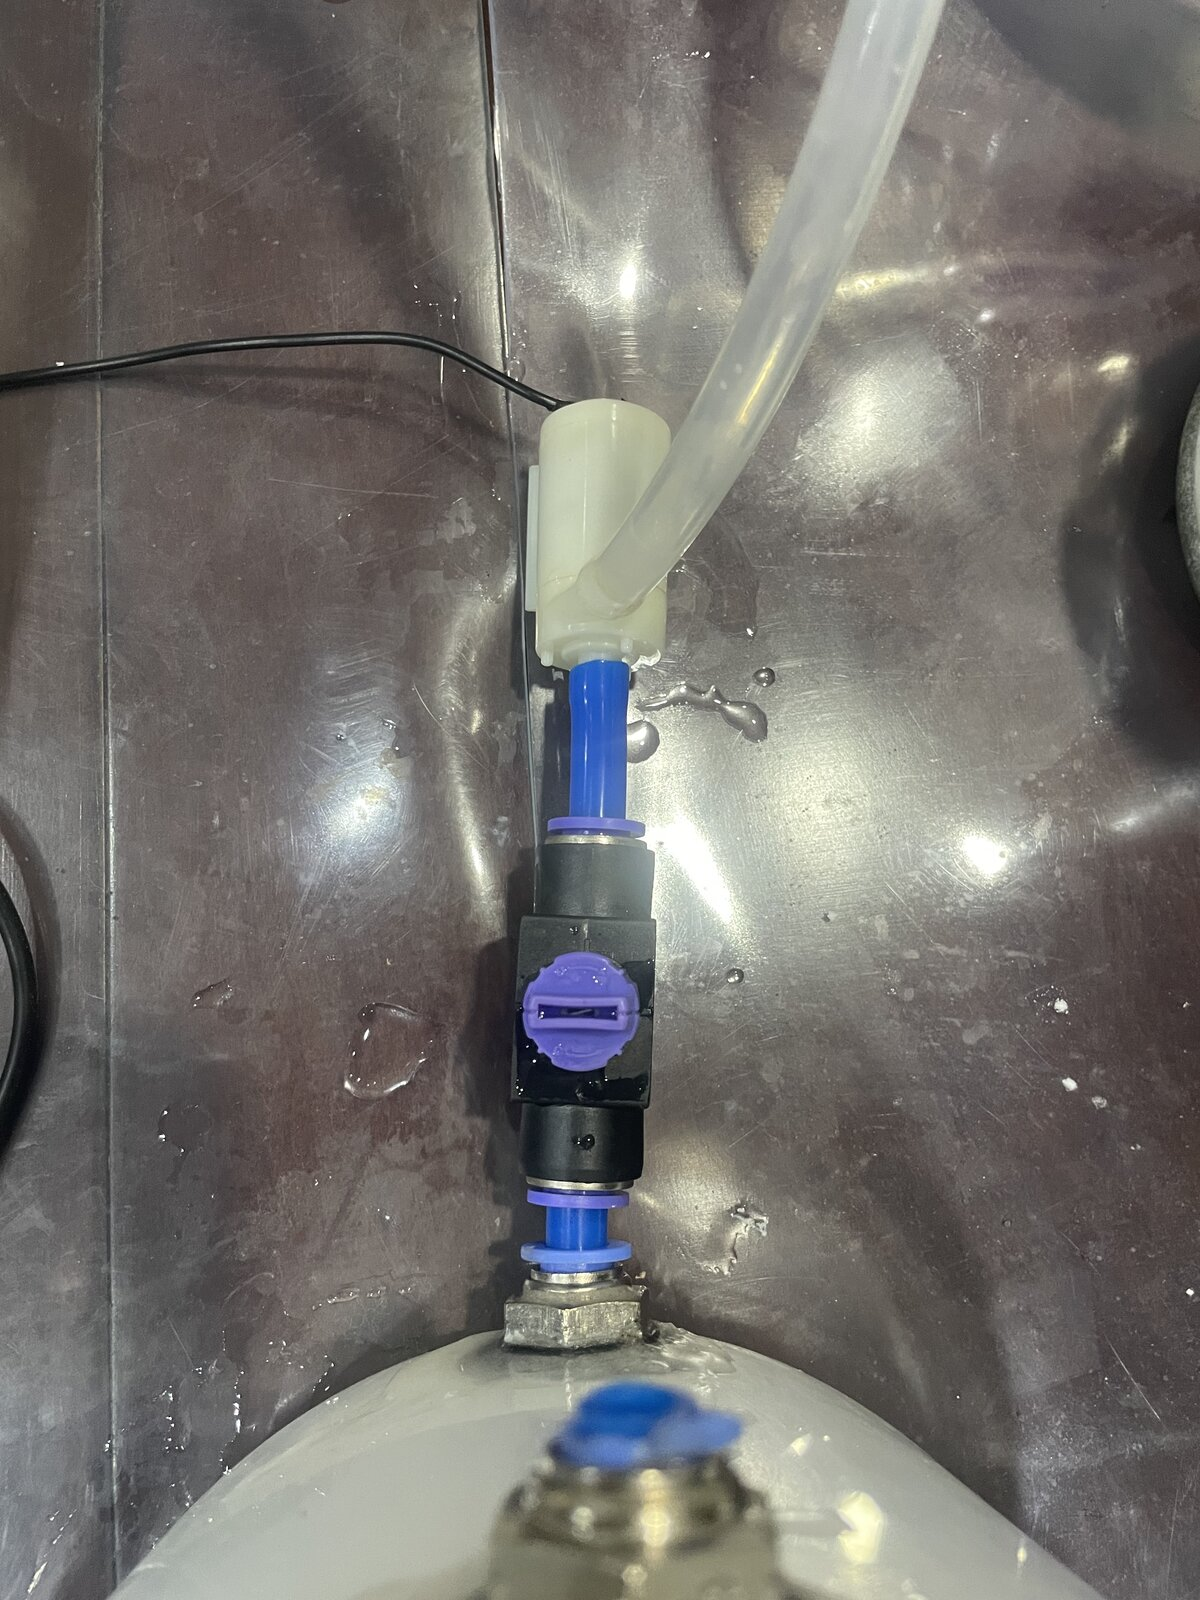
\includegraphics[width=0.45\textwidth]{figuras/fotos/acople_bomba_fuera.jpg}
\caption{Montaje del ensayo integral: salida en la pared del recipiente (abajo), acople rápido y bomba fuera del agua; la manguera transparente sube hacia el balde colector (13 de noviembre de 2026). Elaboración propia.}
\label{fig:acople}
\end{figure}

\begin{figure}[htbp]
\centering
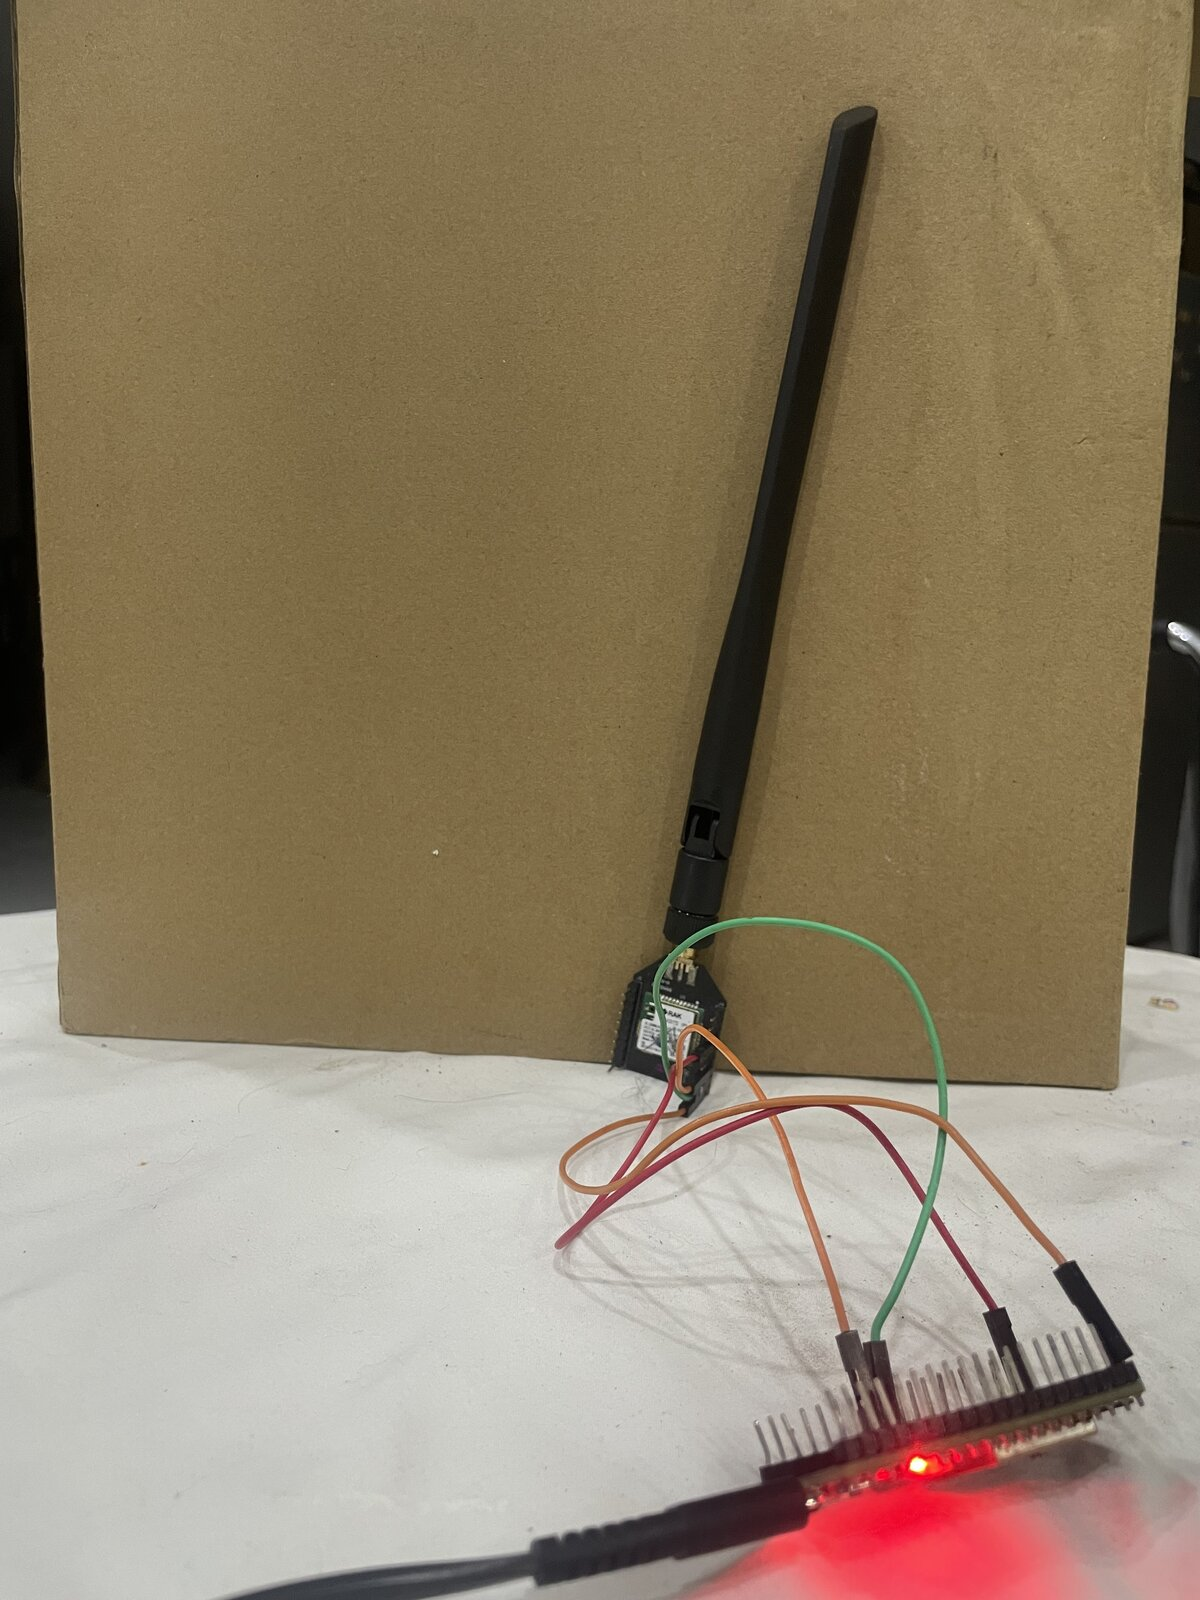
\includegraphics[width=0.55\textwidth]{figuras/fotos/gateway.jpg}
\caption{Gateway GW01: ESP32 con el RAK3272S y su antena (fotografía del 13 de noviembre de 2026). Elaboración propia.}
\label{fig:foto_gateway}
\end{figure}
